\chapter{ShareLaTeX}
\label{ShareLaTeX}
\thispagestyle{empty}

ShareLaTeX è uno strumento assai diffuso all'interno della comunità scientifica e accademica. È un editor di documenti in linguaggio \LaTeX ~che presenta numerose funzionalità che lo caratterizzano rispetto ai normali editor.

\section{Funzionalità}

ShareLaTeX è un'applicazione web che consente agli utenti di registrarsi e creare, importare, modificare e gestire progetti \LaTeX. La caratteristica che contraddistingue ShareLaTeX è l'essere un editor collaborativo. Nel momento in cui l'autore di un documento non è un singolo utente, ma un gruppo, risulta difficile sincronizzare l'andamento del progetto e lo stato dei file con un normale editor \LaTeX. ShareLaTeX consente la condivisione dei documenti con più utenti, ai quali possono essere concessi sia privilegi di lettura che di scrittura. Qualunque modifica apportata al progetto sarà visibile in tempo reale a tutti i collaboratori connessi in quel momento e i file rimarranno consistenti. I progetti conservano inoltre lo storico delle modifiche, quindi è possibile ripristinare ciascun file alla versione precedente, oppure ripristinare un file eliminato.

\section{Interfaccia}
ShareLaTeX offre un'interfaccia utente semplice e immediata. Ogni utente iscritto possiede la sua homepage con i progetti creati, dalla quale può decidere se aprire un progetto esistente o crearne uno nuovo.
\begin{figure}[h]
    \centering
    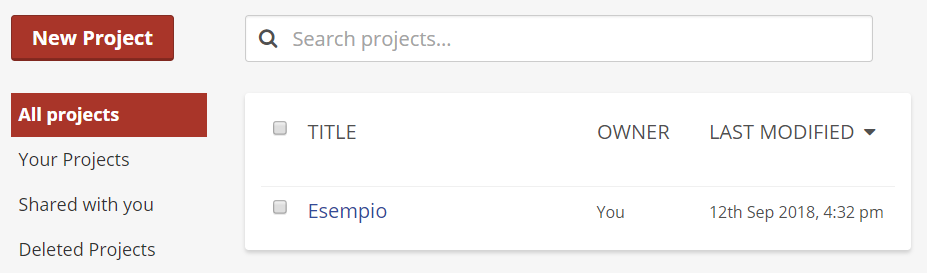
\includegraphics[scale=0.7]{immagini/homepage.PNG}
    \caption{Homepage di ShareLaTeX}
    \label{fig:sharelatex_homepage}
\end{figure}

L'interfaccia dell'editor è anch'essa semplice e divisa in tre parti:
\begin{itemize}
    \item Una colonna di navigazione fra i file del progetto, dalla quale si possono non solo creare nuovi file e cartelle, ma anche importarli da locale o dal web.
    \item La finestra di editor vera e propria, dove l'utente scrive testo e comandi \LaTeX, con evidenziazione della sintassi e consigli sul completamento dei comandi.
    \item La finestra di anteprima del documento, che presenta l'esito della compilazione.
\end{itemize}
\begin{figure}[h]
    \centering
    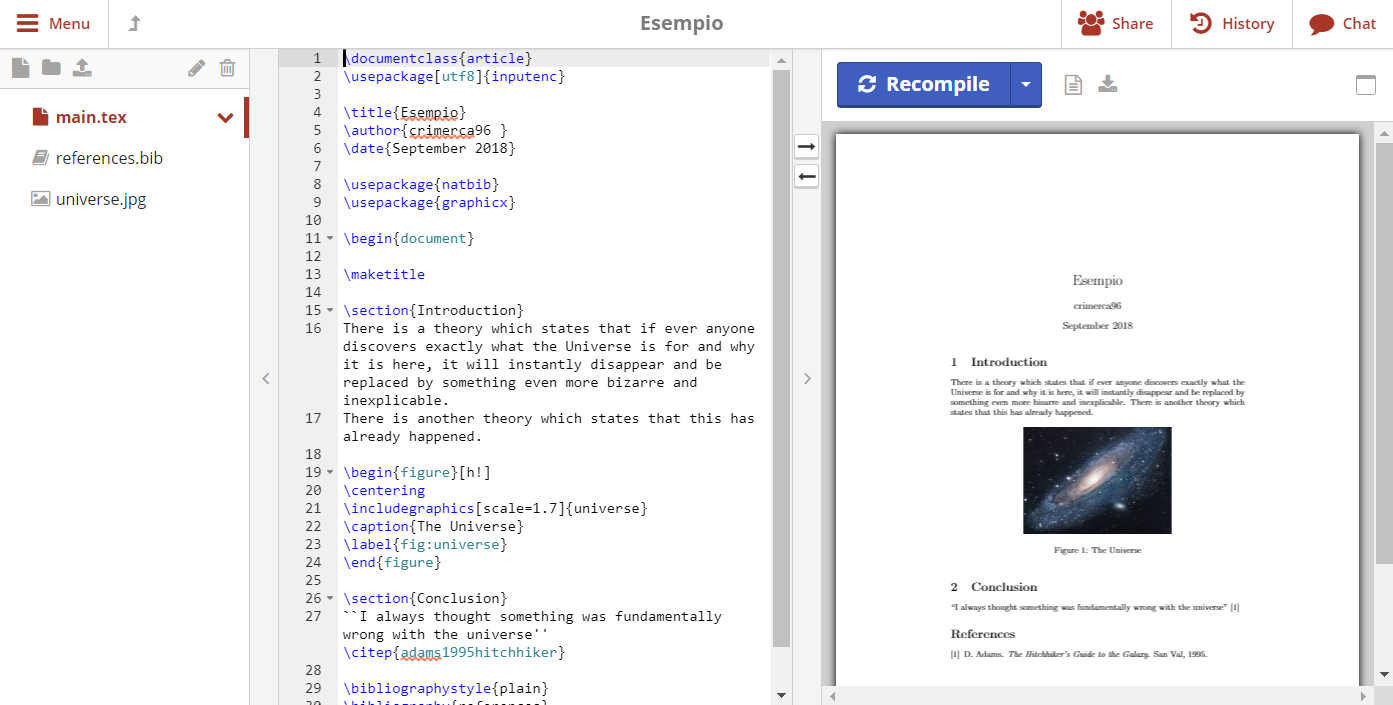
\includegraphics[width=\textwidth]{immagini/editor.PNG}
    \caption{Interfaccia dell'editor di ShareLaTeX}
    \label{fig:sharelatex_editor}
\end{figure}
Nell'editor è inoltre possibile condividere il progetto con altri utenti, visualizzare la cronologia delle modifiche e visualizzare la chat di progetto, mediante i tre pulsanti in alto a destra.
Il pulsante \enquote*{Menu} in alto a sinistra mostra una colonna aggiuntiva dalla quale è possibile:
\begin{itemize}
    \item Scaricare il codice sorgente del progetto e il PDF di output.
    \item Copiare il progetto in un nuovo progetto.
    \item Contare le parole.
    \item Selezionare uno fra i compilatori disponibili: pdf\LaTeX, \LaTeX, Xe\LaTeX e Lua\LaTeX.
    \item Selezionare il documento principale da cui iniziale la compilazione.
    \item Indicare il linguaggio di scrittura per la correzione dello spelling.
    \item Attivare o disattivare l'auto-completamento del testo, l'auto-chiusura delle parentesi e il controllo del codice.
    \item Selezionare il tema ella schermata dell'editor e la dimensione del font.
    \item Mostrare le scorciatoie da tastiera dell'editor.
\end{itemize}

\section{Database}
ShareLaTeX necessita di due DBMS per funzionare: MongoDB e Redis. In seguito si presentano tali servizi, mettendo in luce i loro punti di forza.

\subsection{MongoDB}
MongoDB è un DBMS non relazionale, anche detto NoSQL. È un progetto open source con licenza GNU AGPL v3.0. Anziché essere basato su tabelle e dipendenze fra queste, MongoDB utilizza il modello a documenti. Questi consentono di strutturare i dati in maniera efficiente da processare per le macchine, ma allo stesso tempo naturale e facile per l'essere umano da leggere. DBMS relazionali, specialmente se di grandi dimensioni, possono risultare difficili da comprendere, da aggiornare, inefficienti e spesso gli sviluppatori devono modellare le proprie applicazioni sulle esigenze del DBMS. MongoDB invece si adatta alle esigenze di chi sviluppa, concedendo loro di memorizzare dati in maniera più libera, senza la preoccupazione che un piccolo cambiamento possa compromettere lo stato della base di dati. Inoltre MongoDB può nativamente coordinare molteplici server per immagazzinare dati. È quindi definito \enquote*{distributed database}. È tollerante ai guasti, qualora siano stati previsti server secondari ridondanti. È scalabile, ovvero può immagazzinare dati in più server. Infine è possibile migrare facilmente i database, in modo da conservare i dati vicino agli utenti per garantire accessi veloci.

\subsection{Redis}
Redis è un DBMS non relazionale, anche detto NoSQL. È un progetto open source con licenza BSD 3-Clause. Redis è un archivio di strutture dati, utilizzato sia come database che come meccanismo di caching. Infatti il punto di forza di Redis è la velocità, perché è funziona completamente in memoria RAM ed è scritto in C. Utilizza strutture dati predefinite per migliorare le performance: list, sets, sorted sets, hashes, hyperloglogs, bitmaps, geospatial indexes, bitfields, streams e strings. Redis, oltre ad essere completamente \enquote*{in-memory}, permette la persistenza dei dati e un'alta disponibilità grazie a repliche e backup.


\section{Sviluppo e distribuzione}
ShareLaTeX è un'azienda fondata da Henry Oswald e James Allen. Il software ha licenza GNU AGPL v3.0 e il codice sorgente è liberamente accessibile su GitHub (\url{github.com/sharelatex}). Nel corso degli anni la community ha contribuito alla crescita e al miglioramento della piattaforma. La versione online di ShareLaTeX propone diversi piani di abbonamento all'utente, flessibili su base mensile e annuale, con prezzo dimezzato per gli studenti. I vari abbonamenti differiscono per il numero di collaboratori per progetto e per la presenza delle funzionalità aggiuntive di sincronizzazione con Dropbox e GitHub.

Gli sviluppatori hanno fornito una guida per l'installazione e configurazione dei ShareLaTeX, disponibile all'indirizzo \url{github.com/sharelatex/sharelatex/wiki}. Tale guida è stata usata come riferimento principale per lo svolgimento di questo progetto. Gli sviluppatori hanno inoltre fornito un immagine aggiornata e funzionante del sistema per la piattaforma Docker all'indirizzo \url{hub.docker.com/u/sharelatex/}.

\section{Overleaf v2}
Il 20 luglio 2017 ShareLaTeX annuncia la fusione con Overleaf, un altro software per l'editing collaborativo di progetti \LaTeX. Dall'unione nasce Overleaf v2. Dal 4 settembre 2018 ShareLaTeX non è più disponibile e tutti gli account creati sono stati esportati sulla nuova piattaforma all'indirizzo \url{v2.overleaf.com}. Il team ha comunque dichiarato che ShareLaTeX continuerà a crescere e ad essere open source. L'interfaccia della homepage e dell'editor sono le medesime di ShareLaTeX, con qualche cambiamento estetico. Inoltre è possibile scrivere utilizzando la nuova funzionalità chiamata \enquote*{Rich text}, che consente di visualizzare nella finestra di scrittura un'interfaccia più user-friendly, adatta a chi non è esperto di \LaTeX ~e dei suoi comandi.
\begin{figure}[h]
    \centering
    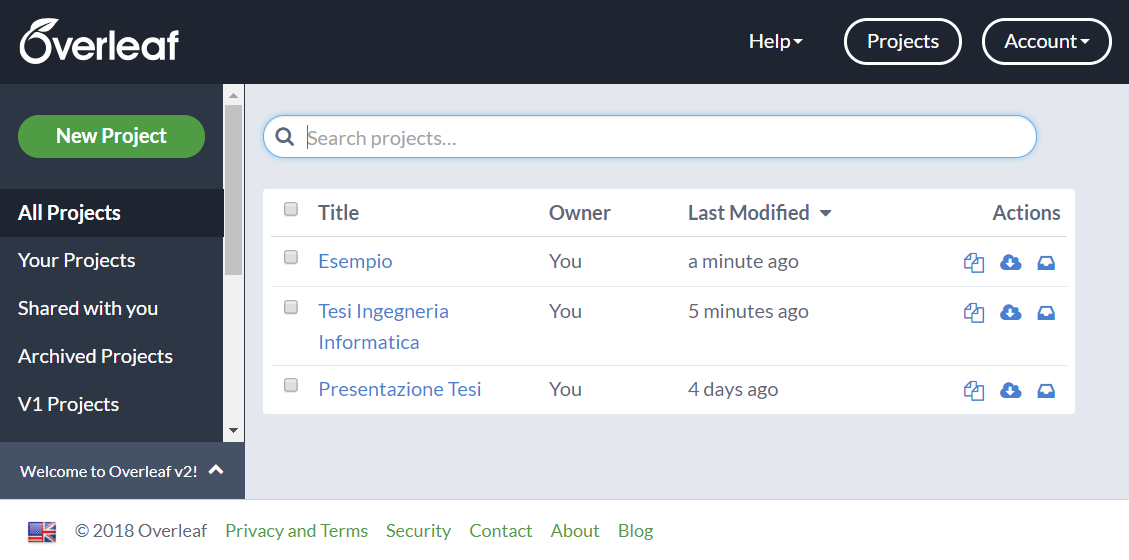
\includegraphics[width=\textwidth]{immagini/overleaf_homepage.PNG}
    \caption{Homepage di Overleaf v2}
    \label{fig:overleaf_homepage}
\end{figure}
\begin{figure}[h]
    \centering
    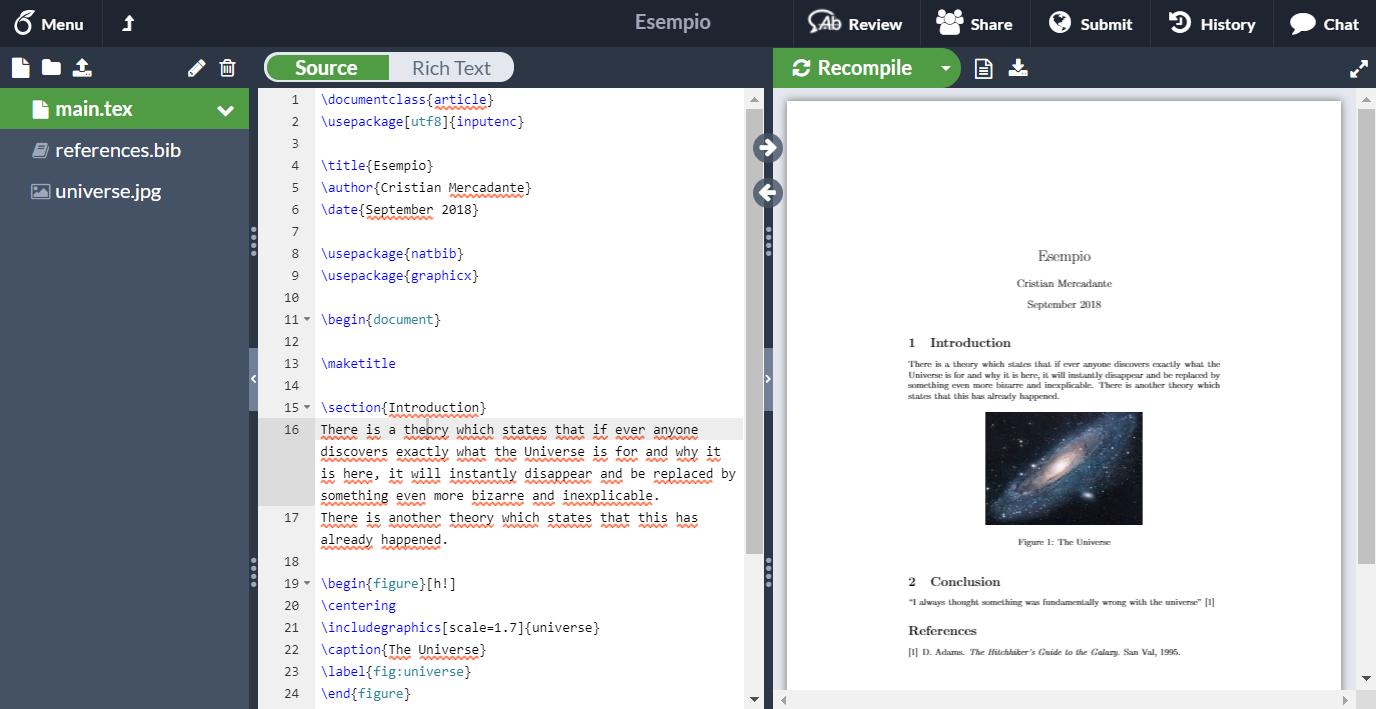
\includegraphics[width=\textwidth]{immagini/overleaf_editor.PNG}
    \caption{Interfaccia dell'editor di Overleaf v2}
    \label{fig:overleaf_editor}
\end{figure}

